%
% chapter.tex -- Kapitel über Algorithmen
%
% (c) 2019 Prof Dr Andreas Müller, Hochschule Rapperswil
%
\chapter{Schnelle Wavelet-Algorithmen
\label{chapter:algo}}
\lhead{Schnelle Wavelet-Algorithmen}
Wavelets versprechen einen Signalanalyse, die sich auf jeder Skala auf
die gleiche Art und Weise abspielt.
Die Multiskalen-Analyse gibt dies auf axiomatische Art und Weise wieder.
In jedem der Funktionenräume $V_{j+1}$ sind die hochfrequenten und die 
niederfrequenten Teile der Signale in gleicher Weise auf die 
orthogonalen Unterräume $W_j$ und $V_j$ verteilt.

%
% fast.tex
%
% (c) 2019 Prof Dr Andreas Müller, Hochschule Rapperswil
%
\section{Schnelle Algorithmen
\label{section:fast}}
\rhead{Schnelle Algorithmen}
Die Basisfunktion $\psi_{j,k}$ geben die Details eines Signals nahe bei
$t=k2^{-j}$ mit einer Auflösung von der Grössenordnung $2^{-j}$ wieder.
Je grösser $j$, desto feiner die Auflösung.
Da die $\psi_{j,k}$ nur eine Basis von $W_j$ sind, werden ausserdem die
Basisfunktion $\varphi_{j,k}$ in mindestens einem der Vektorräume
$V_j$ gebraucht.
Ein praktisch nützlicher Analyse-Algorithmus muss die Koeffizienten
\[
\begin{aligned}
a_{j,k}
&=
\langle f, \varphi_{j,k}\rangle
=
\langle f, D_{2^{-j}}T_k\varphi \rangle
&&&&\text{Mittelwerte}
\\
b_{j,k}
&=
\langle f, \psi_{j,k}\rangle
=
\langle f, D_{2^{-j}}T_k\psi \rangle
&&&&\text{Detail}
\end{aligned}
\]
für jedes beliebige Signal $f$ auf effiziente Art berechnen können.
Dabei wird verwendet, dass die Funktionen  $\varphi_{j,k}$ eine
orthonormierte Basis von $V_j$ sind und die $\psi_{j,k}$ eine
orthonormierte Basis von $W_j$.

\begin{figure}
\centering
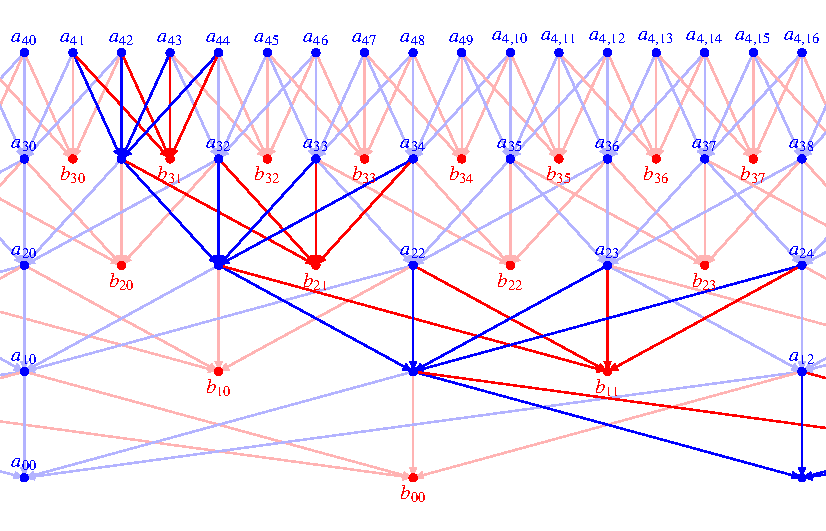
\includegraphics{chapters/7-algo/images/fastalgo.pdf}
\caption{Datenfluss für die Analyse mit vier von $0$ verschiedenen
Koeffizienten $\color{blue}\bar{h}_{-1},\dots,\bar{h}_2$ und
$\color{red}\bar{g}_{-1},\dots,\bar{g}_2$.
Ausgangsdaten für die Analyse sind die Samples $\color{blue}a_{4k}$
in der ersten Zeile.
Durch Anwendung der $\color{blue}h$-Koeffizienten (blaue Linien) können daraus
die Mittelwerte mit gröberer Auflösung $\color{blue}a_{3k}$ gewonnen werden.
Ebenso können durch Anwendung der $\color{red}g$-Koeffizienten (rote Linien)
die Detail-Koeffizienten $\color{red}b_{3k}$ gefunden werden.
Dies wird für jede weitere Detail-Ebene $j$ wiederholt: aus den Koeffizienten
$\color{blue}a_{jk}$ werden mit den $\color{blue}h$-Koeffizienten die
$\color{blue}a_{j+1,k}$ und mit den $\color{red}g$-Koeffizienten die
$\color{red}b_{j+1,k}$ bestimmt.
\label{algo:image:fastalgo}}
\end{figure}

Ein Schlüsselelement einer Multiskalen-Analyse ist die Skalierungsrelation
\begin{align}
\varphi(t) &= \sqrt{2} \sum_{l\in\mathbb Z} h_l \varphi(2t-l)
\notag
\intertext{oder mit den Operatoren $D$ und $T$ geschrieben:}
\varphi    &= \sum_{l\in\mathbb Z} h_l D_{\frac12}T_l\varphi.
\label{algo:formel:phiscale}
\end{align}
Da die Skalierung $D_{\frac12}$ jeden der Vektorräume $V_j$ isometrisch
auf $V_{j+1}$ abbildet, wird daraus eine Skalierungsrelation für alle
Basisfunktionen $\varphi_{j,k}$, die durch Anwendung des Operators
$D_{2^{-j}}T_k$ auf \eqref{algo:formel:phiscale} gefunden werden kann:
\begin{equation}
\varphi_{j,k}
=
D_{2^{-j}}T_k\varphi
=
\sum_{l\in\mathbb Z} h_l D_{2^{-j}} T_k D_{\frac12}T_l \varphi
=
\sum_{l\in\mathbb Z} h_l D_{2^{-j}} D_{\frac12}T_{2k}T_l \varphi
=
\sum_{l\in\mathbb Z} h_l D_{2^{-j-1}} T_{l+2k} \varphi
=
\sum_{l\in\mathbb Z} h_l \varphi_{j+1,l+2k}
\label{fast:phirelation}
\end{equation}
Im zweitenletzten Schritt haben wir die Vertauschungsrelation für 
$D_{\frac12}$ und $T_k$ verwendet.
Ausserdem folgt aus der Tatsache, dass $W_j\subset V_{j+1}$ ist,
dass die Basisfunktionen $\psi_{j,k}$ der Orthonormalbasis von $W_j$
Linearkombinationen der Funktionen $\varphi_{j+1,l}$ sein müssen,
folgt die Relation
\[
\psi(t) = \sqrt{2}\sum_{l\in\mathbb Z} g_l \varphi(2t-l),
\]
für das Mutter-Wavelet.
Wieder mit Hilfe der Skalierungs-Isometrien $D_{\frac12}$ folgt eine
entsprechende Relation
\begin{equation}
\psi_{j,k}
=
\sum_{l\in\mathbb Z} g_l D_{2^{-j-1}}T_{l+2k}\varphi
=
\sum_{l\in\mathbb Z} g_l \varphi_{j+1,l+2k}
\label{fast:psirelation}
\end{equation}
für die skalierten und verschobenen Wavelets.

Wendet man die Relationen \eqref{fast:phirelation} und \eqref{fast:psirelation}
auf das Signal $f$ an, indem man das Skalarprodukt mit $f$ bildet,
findet man die Beziehungen
\begin{align}
a_{j,k}
=
\langle f,\varphi_{j,k} \rangle
&=
\sum_{l\in\mathbb Z} \bar{h}_l \langle f,\varphi_{j+1,l+2k}\rangle
=
\sum_{l\in\mathbb Z} \bar{h}_l a_{j+1,l+2k}
\label{fast:akoefgleichung}
\\
b_{j,k}
=
\langle f,\psi_{j,k} \rangle
&=
\sum_{l\in\mathbb Z} \bar{g}_l \langle f,\varphi_{j+1,l+2k}\rangle
=
\sum_{l\in\mathbb Z} \bar{g}_l a_{j+1,l+2k}
\label{fast:bkoefgleichung}
\end{align}
für die Koeffizienten $b_{j,k}$ und $a_{j,k}$.
Die Formeln drücken die Wavelet-Koeffizienten für die Auflösung $j$ durch
die Wavelet-Koeffizienten für die Auflösung $j+1$ aus.
Sobald die Koeffizienten $a_{N,k}$ bekannt sind, können alle Koeffizienten
$a_{j,k}$ mit $j<N$, berechnet werden.

Bleibt die Frage zu klären, woher denn die Koeffizienten $a_{N,k}$ in einer
praktischen Anwendung der Wavelet-Transformation kommen.
Für grosses $j$ ist die Funktion $\varphi_{j,k}$ in der Nähe von $2^{-j}k$
konzentriert.
Ändert das Signal $f$ in einer Umgebung von $2^{-j}k$ nur wenig, kann man
\begin{equation*}
a_{j,k}
=
\langle f,\varphi_{j,k}\rangle
=
\int_{-\infty}^\infty f(t)\, \varphi_{j,k}(t)\,dt
\simeq
f(2^{-j}k)
\int_{-\infty}^\infty \varphi_{j,k}(t)\,dt
\end{equation*}
approximieren.
Bis auf einen möglichen skalaren Faktor gegeben durch das Integral, sind
die Koeffizienten $a_{j,k}$ für genügend grosses $j$ also durch
Sample-Werte $f(2^{-j}k)$ ausreichend genau approximiert.

\begin{beispiel}
Die Skalierungsrelation des Haar-Wavelets hat die Koeffizienten
$h_0=h_1=1$, $g_0=1$ und $g_1=-1$.
Die Berechnung der Koeffizienten gemäss \eqref{fast:akoefgleichung}
und \eqref{fast:bkoefgleichung} führt auf das folgende Berechnungsschema:
\[
\xymatrix{
\dots
	&a_{j,-2} \ar[d] \ar[dr]
		&a_{j,-1} \ar@[red][d]^{\color{red}\cdot (-1)} \ar[dl]
			&a_{j,0} \ar[d] \ar[dr]
				&a_{j,1} \ar@[red][d]^{\color{red}\cdot (-1)} \ar[dl]
					&a_{j,2} \ar[d] \ar[dr]
						&a_{j,3} \ar@[red][d]^{\color{red}\cdot (-1)} \ar[dl]
							&\dots
\\
\dots
	&a_{j-1,-1} \ar@[red][d]^{\color{red}\cdot(-1)}
		&b_{j-1,-1}
			&a_{j-1,0}\ar[d] \ar[drr]
				&b_{j-1,0}
					&a_{j-1,1} \ar@[red][d]^{\color{red}\cdot (-1)} \ar[dll]
						&b_{j-1,1}
							&\dots
\\
\dots &b_{j-2,-1} 
		&
			&a_{j-2,0} \ar[d] \ar[drrrr]
				&
					&b_{j-2,0}
						&
							&\dots \ar[dllll]
\\
\dots &
		&
			&a_{j-3,0}
				&
					&
						&
							&\dots
}
\]
Wo immer zwei Pfeile zusammenkommen, müssen die Terme, von denen die
Pfeile ausgehen, summiert werden.
Rote Pfeile multiplizieren die Ausgangsterme zusätzlich mit $-1$.
\end{beispiel}





%
% synthese.tex -- synthese 
%
% (c) 2019 Prof Dr Andreas Müller, Hochschule Rapperswil
%
\section{Schnelle Synthese\label{section:schnelle-synthese}}
\rhead{Schnelle Synthese}
Im vorangegangenen Abschnitt wurde dargestellt, wie die Waveletkoeffizienten
$a_{j,k}$ mit einem schnellen Algorithmus aus den Waveletkoeffizienten
$a_{j+1,k}$ gewonnen werden können.
Dabei spielte die Skalierungsrelation für das Vaterwavelet $\varphi$ und die
Darstellung des Mutterwavelet $\psi$ als Linearkombination von $\varphi_{1,k}$
die entscheidende Rolle.
Die Orthogonalität der Basisvektoren war bisher nicht von Bedeutung.

Die Umkehrung einer linearen Transformation erfordert die
Invertierung einer Matrix, ein im Allgmeinen aufwendiger Prozess.
Doch für orthonormierte Basen ist die Umkehrung einfach.
In diesem Falle ist die Koordinationentransformationsmatrix
orthogonal und die inverse Matrix ist die Transponierte.
Da die aus einer Multiskalenanalyse hervorgegangenen Waveletbasen
orthonormiert sind, erwarten wir daher eine ebenfalls leicht zu
berechnende schnelle Umkehrtransformation.
Sie soll im Folgenden dargestellt werden.

Die schnelle Wavelettransformation erzeugt die Detailkoeffizienten
$b_{jk}$ aus den Samples $a_{Nk}$.
Dies entspricht einem Basiswechsel von $\varphi_{N,k}$ zu den
Vektoren $\psi_{j,k}$ für $j<N$.
Wir wollen diesen Basiswechsel als Transformationsmatrix für 
die Waveletkoeffizienten ausdrücken und schliesslich auch invertieren.

%
% Basiswechsel zwischen orthonormierten Basen
%
\subsection{Basiswechsel und Koordinatentransformationsmatrix}
Zunächst erinnern wir an die abstrakte Konstruktion der
Transformationsmatrix für die Koordinaten bei einem Basiswechsel.
Zu diesem Zweck seien in einem Vektorraum $V$ zwei Basen
$\mathcal{B}=\{b_i\in V\}$ und $\mathcal{C}=\{c_i\in V\}$ vorgegeben.
Gesucht wird die Umrechnung von Koordinaten bezüglich der Basis
$\mathcal{B}$ in Koordinaten bezüglich der Basis $\mathcal{C}$.

Da $\mathcal{C}$ eine Basis ist, lassen sich die Vektoren $b_i$ als
Linearkombinationen
\begin{equation}
b_i = \sum_{j}  t_{ji}c_j
\label{algo:basiswechsel}
\end{equation}
der $c_j$ schreiben.
Ein beliebiger Vektor $v\in V$ habe in der Basis $\mathcal{B}$ die
Koordinaten $\xi_i$, er lässt sich also als Linearkombination
\[
v=\sum_{i} \xi_i b_i
\]
schreiben.
Durch Substitution der Ausdrücke \eqref{algo:basiswechsel} für $b_i$
lassen sich die Koordinaten von $v$ in der Basis $\mathcal{C}$ finden:
\[
\sum_{i} \xi_i b_i
=
\sum_{i,j} \underbrace{t_{ji}\xi_i}_{\displaystyle=\eta_j} c_j
\qquad\Rightarrow\qquad
\eta_j = \sum_{i} t_{ji} \xi _i.
\]
Die Notation ist so gewählt, dass die Matrix $T$ mit Einträgen $t_{ji}$ 
den Vektor $\xi$ der Koordinaten $\xi_i$ mittels eines Produktes $T\xi$
in den Vektor $\eta$ der Koordinaten $\eta_j$ der Koordinaten bezüglich
der Basis $\mathcal{C}$ transformiert.

\subsection{Transformationsmatrix für Waveletkoeffizienten}
Im Waveletkontext liefert die Skalierungsrelation den Zusammenhang
zwischen den verschiedenen Basen.
Die Multiskalenanalyse verspricht, dass sich jeder der Vektorräume
$V_{j+1}$ auf zwei Arten mit einer Basis ausstatten lässt.
Einerseits bilden die Vektoren $D_{j+1}T_k\varphi$ eine orthonormierte
Basis von $V_{j+1}$.
Andererseits lässt sich $V_{j+1}$ schreiben als orthogonale Summe
$V_j\oplus W_j$, in der jeder Summand eine orthonormierte Basis hat.
In $V_j$ ist des die Basis der Vektoren $D_{2^{-j}}T_k\varphi$, in $W_j$
sind es die $D_{2^{-j}}T_k\psi$.

Die Skalierungsrelation für das Vaterwavelet und die Darstellung des
Mutterwavelets liefern die Beziehungen
\begin{align*}
\varphi_{j,k} &= \sum_{l} h_{l}\varphi_{j+1,l+2k}
\qquad\text{und}
\\
\psi_{j,k} &= \sum_{l} g_{l} \varphi_{j+1,l+2k}.
\end{align*}

Im Abschnitt~\ref{section:fast} haben wir daraus die Formeln für
die schnelle Wavelettransformation abgeleitet:
\begin{align*}
a_{j,k} &= \sum_{l} \bar{h}_l a_{j+1,l+2k} \qquad\text{und}
\\
b_{j,k} &= \sum_{l} \bar{g}_l a_{j+1,l+2k}
\end{align*}
abgeleitet.
Die Koeffizienten $a_{\cdot,\cdot}$ und $b_{\cdot,\cdot}$ entsprechen
den Koordinaten $\xi_{\cdot}$ und $\eta_{\cdot}$ weiter oben.

An der Verschiebungsposition $k$ sind in der Basis von $V_{j+1}$ 
primär die Koffizienten um $a_{j+1,2k}$ herum massgebend.
In $V_j$ und $W_j$ sind es dagegeben die Koeffizienten $a_{j,k}$ und
$b_{j,k}$.
Es liegt daher nahe, die Basisvektoren in $V_j$ und $W_j$ zu mischen
und die Reihenfolge
\[
\dots    
\varphi_{j,k-1},\psi_{j,k-1},
\varphi_{j,k},\psi_{j,k},
\varphi_{j,k+1},\psi_{j,k+1},
\varphi_{j,k+2},\psi_{j,k+2},
\dots
\]
zu verwenden.
Für die Umrechnung der Koeffzienten $a_{j+1,k}$ in $a_{j,k}$ und $b_{j,k}$
ist dann die Matrix \eqref{fast:transmatrix} anzuwenden.
Der oben beschriebene schnelle Waveletalgorithmus implementiert diese
Matrixmultiplikation.
\begin{figure}
\begin{gather}
\bgroup
\def\arraystretch{1.5}
\begin{tabular}{>{$\mathstrut}c<{$}|
>{$}c<{$}
>{$}c<{$}
>{$}c<{$}
>{$}c<{$}
>{$}c<{$}
>{$}c<{$}
>{$}c<{$}
>{$}c<{$}
>{$}c<{$}
>{$}c<{$}}
        &\dots &a_{j+1,-2}  &a_{j+1,-1}  &a_{j+1,0}   &a_{j+1,1}   &a_{j+1,2}   &a_{j+1,3}   &a_{j+1,4}&a_{j+1,5}&\dots \\
\hline
\vdots  &\ddots&\vdots      &\vdots      &\vdots      &\vdots      &\vdots      &\vdots      &\vdots   &\vdots   &\ddots\\
{\color{blue}a_{j,-2}}&\dots &\begin{picture}(0,0)\color{blue}\drawline(-30,-5)(55,-5)(55,10)(-30,10)\end{picture}
                \bar{h}_2   &\bar{h}_3   &\bar{h}_4   &\bar{h}_5   &\bar{h}_6   &\bar{h}_7   &\bar{h}_8&\bar{h}_9&\dots \\
{\color{red}b_{j,-2}}&\dots &\begin{picture}(0,0)\color{red}\drawline(-30,-5)(55,-5)(55,10)(-30,10)\end{picture}
                \bar{g}_2   &\bar{g}_3   &\bar{g}_4   &\bar{g}_5   &\bar{g}_6   &\bar{g}_7   &\bar{g}_8&\bar{g}_9&\dots \\
{\color{blue}a_{j,-1}}&\dots &\begin{picture}(0,0)\color{blue}\drawline(-10,-5)(125,-5)(125,10)(-10,10)(-10,-5)\end{picture}
                \bar{h}_0   &\bar{h}_1   &\bar{h}_2   &\bar{h}_3   &\bar{h}_4   &\bar{h}_5   &\bar{h}_6&\bar{h}_7&\dots \\
{\color{red}b_{j,-1}}&\dots &\begin{picture}(0,0)\color{red}\drawline(-10,-5)(125,-5)(125,10)(-10,10)(-10,-5)\end{picture}
                \bar{g}_0   &\bar{g}_1   &\bar{g}_2   &\bar{g}_3   &\bar{g}_4   &\bar{g}_5   &\bar{g}_6&\bar{g}_7&\dots \\
{\color{blue}a_{j, 0}}&\dots &\bar{h}_{-2}&\bar{h}_{-1}&\begin{picture}(0,0)\color{blue}\drawline(-10,-5)(118,-5)(118,10)(-10,10)(-10,-5)\end{picture}
                                          \bar{h}_0   &\bar{h}_1   &\bar{h}_2   &\bar{h}_3   &\bar{h}_4&\bar{h}_5&\dots \\
{\color{red}b_{j, 0}}&\dots &\bar{g}_{-2}&\bar{g}_{-1}&\begin{picture}(0,0)\color{red}\drawline(-10,-5)(118,-5)(118,10)(-10,10)(-10,-5)\end{picture}
                                          \bar{g}_0   &\bar{g}_1   &\bar{g}_2   &\bar{g}_3   &\bar{g}_4&\bar{g}_5&\dots \\
{\color{blue}a_{j, 1}}&\dots &\bar{h}_{-4}&\bar{h}_{-3}&\bar{h}_{-2}&\bar{h}_{-1}&\begin{picture}(0,0)\color{blue}\drawline(-10,-5)(116,-5)(116,10)(-10,10)(-10,-5)\end{picture}
                                                                    \bar{h}_0   &\bar{h}_1   &\bar{h}_2&\bar{h}_3&\dots \\
{\color{red}b_{j, 1}}&\dots &\bar{g}_{-4}&\bar{g}_{-3}&\bar{g}_{-2}&\bar{g}_{-1}&\begin{picture}(0,0)\color{red}\drawline(-10,-5)(116,-5)(116,10)(-10,10)(-10,-5)\end{picture}
                                                                    \bar{g}_0   &\bar{g}_1   &\bar{g}_2&\bar{g}_3&\dots \\
{\color{blue}a_{j, 2}}&\dots &\bar{h}_{-6}&\bar{h}_{-5}&\bar{h}_{-4}&\bar{h}_{-3}&\bar{h}_{-2}&\bar{h}_{-1}&\begin{picture}(0,0)\color{blue}\drawline(70,-5)(-10,-5)(-10,10)(70,10)\end{picture}
              \bar{h}_0&\bar{h}_1&\dots \\
{\color{red}b_{j, 2}}&\dots &\bar{g}_{-6}&\bar{g}_{-5}&\bar{g}_{-4}&\bar{g}_{-3}&\bar{g}_{-2}&\bar{g}_{-1}&\begin{picture}(0,0)\color{red}\drawline(70,-5)(-10,-5)(-10,10)(70,10)\end{picture}
              \bar{g}_0&\bar{g}_1&\dots \\
\vdots  &\ddots&\vdots      &\vdots      &\vdots      &\vdots      &\vdots      &\vdots      &\vdots   &\vdots   &\ddots\\
\end{tabular}
\egroup
\label{fast:transmatrix}
\\[10pt]
%\end{equation}
%\caption{Darstellung der Wavelettransformation als Transformationsmatrix.
%Die Koeffizienten mit Indizes $0$ bis $3$, die bei einem \texttt{db2}-Wavelet
%von $0$ verschieden sind, sind farblich hervorgehoben, dadurch wird die
%Struktur besser erkennbar.
%Alternierende Zeilen sind bis auf eine Verschiebung um 2 identisch,
%die Matrix beschreibt daher zwei Faltungsfilter mit Koeffizienten
%$\bar{h}_k$ und $\bar{g}_k$.
%\label{algo:vorwaertstransformation}}
%\end{figure}
%\begin{figure}
%\begin{equation}
\bgroup
\def\arraystretch{1.5}
\begin{tabular}{>{$}c<{$}|
>{$}c<{$}
>{$}c<{$}
>{$}c<{$}
>{$}c<{$}
>{$}c<{$}
>{$}c<{$}
>{$}c<{$}
>{$}c<{$}
>{$}c<{$}
>{$}c<{$}
>{$}c<{$}
>{$}c<{$}}
          &\dots &{\color{blue}a_{j,-2}}&{\color{red}b_{j,-2}}&{\color{blue}a_{j,-1}}&{\color{red}b_{j,-1}}&{\color{blue}a_{j,0}}&{\color{red}b_{j,0}}&{\color{blue}a_{j,1}}&{\color{red}b_{j,1}}&{\color{blue}a_{j,2}}&{\color{red}b_{j,2}}&\dots \\
\hline
\vdots    &\ddots&\vdots  &\vdots  &\vdots  &\vdots  &\vdots &\vdots &\vdots &\vdots &\vdots &\vdots &\ddots\\
a_{j+1,-2}&\dots &\begin{picture}(0,0)\color{darkgreen}\drawline(-10,-5)(105,-5)(105,10)(-10,10)(-10,-5)\end{picture}
                  h_{ 2}  &g_{ 2}  &h_{ 0}  &g_{ 0}  &h_{-2} &g_{-2} &h_{-4} &g_{-4} &h_{-6} &g_{-6} &\dots \\
a_{j+1,-1}&\dots &\begin{picture}(0,0)\color{orange}\drawline(-10,-5)(105,-5)(105,10)(-10,10)(-10,-5)\end{picture}
                  h_{ 3}  &g_{ 3}  &h_{ 1}  &g_{ 1}  &h_{-1} &g_{-1} &h_{-3} &g_{-3} &h_{-5} &g_{-5} &\dots \\
a_{j+1, 0}&\dots &h_{ 4}  &g_{ 4}  &\begin{picture}(0,0)\color{darkgreen}\drawline(-10,-5)(98,-5)(98,10)(-10,10)(-10,-5)\end{picture}
                  h_{ 2}  &g_{ 2}  &h_{ 0} &g_{ 0} &h_{-2} &g_{-2} &h_{-4} &g_{-4} &\dots \\
a_{j+1, 1}&\dots &h_{ 5}  &g_{ 5}  &\begin{picture}(0,0)\color{orange}\drawline(-10,-5)(98,-5)(98,10)(-10,10)(-10,-5)\end{picture}
                  h_{ 3}  &g_{ 3}  &h_{ 1} &g_{ 1} &h_{-1} &g_{-1} &h_{-3} &g_{-3} &\dots \\
a_{j+1, 2}&\dots &h_{ 6}  &g_{ 6}  &h_{ 4}  &g_{ 4}  &\begin{picture}(0,0)\color{darkgreen}\drawline(-10,-5)(90,-5)(90,10)(-10,10)(-10,-5)\end{picture}
                  h_{ 2} &g_{ 2} &h_{ 0} &g_{ 0} &h_{-2} &g_{-2} &\dots \\
a_{j+1, 3}&\dots &h_{ 7}  &g_{ 7}  &h_{ 5}  &g_{ 5}  &\begin{picture}(0,0)\color{orange}\drawline(-10,-5)(90,-5)(90,10)(-10,10)(-10,-5)\end{picture}
                  h_{ 3} &g_{ 3} &h_{ 1} &g_{ 1} &h_{-1} &g_{-1} &\dots \\
a_{j+1, 4}&\dots &h_{ 8}  &g_{ 8}  &h_{ 6}  &g_{ 6}  &h_{ 4} &g_{ 4} &\begin{picture}(0,0)\color{darkgreen}\drawline(-10,-5)(90,-5)(90,10)(-10,10)(-10,-5)\end{picture}
                  h_{ 2} &g_{ 2} &h_{ 0} &g_{ 0} &\dots \\
a_{j+1, 5}&\dots &h_{ 9}  &g_{ 9}  &h_{ 7}  &g_{ 7}  &h_{ 5} &g_{ 5} &\begin{picture}(0,0)\color{orange}\drawline(-10,-5)(90,-5)(90,10)(-10,10)(-10,-5)\end{picture}
                  h_{ 3} &g_{ 3} &h_{ 1} &g_{ 1} &\dots \\
\vdots    &\ddots&\vdots  &\vdots  &\vdots  &\vdots  &\vdots &\vdots &\vdots &\vdots &\vdots &\vdots &\ddots\\
\end{tabular}
\egroup
\label{fast:rueckmatrix}
\end{gather}
%\end{equation}
\caption{Darstellung der Wavelettransformation~\eqref{fast:transmatrix}
und der Rücktransformation~\eqref{fast:rueckmatrix} als Transformationsmatrizen.
Die Koeffizienten mit Indizes $0$ bis $3$, die bei einem \texttt{db2}-Wavelet
von $0$ verschieden sind, sind farblich hervorgehoben, dadurch wird die
Struktur besser erkennbar.
Alternierende Zeilen sind bis auf eine Verschiebung um 2 identisch,
beide Matrizen beschreiben daher zwei Faltungsfilter mit Koeffizienten
$\bar{h}_k$ und $\bar{g}_k$, die für die Rücktransformation nur 
konjugiert und etwas anders angeordnet sind.
\label{algo:transformation}}
\end{figure}
%
% invertierung der Transformation
%
\subsection{Invertierung}
Wir nehmen jetzt zusätzlich an, dass die Basen $\mathcal{B}$ und $\mathcal{C}$
orthonormiert sind, eine Voraussetzung, die für die skalierten Mutter- und
Vaterwavelets einer Multiskalenanalyse erfüllt ist.
Es gilt also
\[
\begin{aligned}
\langle b_i,b_j\rangle &=\delta_{ij}\;\forall i,j
&&\text{und}
&
\langle c_i,c_j\rangle &=\delta_{ij}\;\forall i,j.
\end{aligned}
\]
%Auch diese Bedingung ist für die Basen, die aus einer Multiskalenanalyse hervorgehen, erfüllt.
Die Koeffizienten $t_{ji}$ waren definiert durch die
Formel~\eqref{algo:basiswechsel}.
Die Orthogonalitätsbedingungen für die Vektoren $b_i$ werden damit
\[
\langle b_i,b_k\rangle
=
\biggl\langle
\sum_{j}t_{ji}c_j,\sum_{l}t_{lk}c_l
\biggr\rangle
=
\sum_{j,l} t_{ji}\bar{t}_{lk}
\underbrace{\langle c_j,c_l\rangle}_{\displaystyle=\delta_{jl}}
=
\sum_{j} t_{ji}\bar{t}_{jk}.
\]
In Matrixschreibweise ist dies
\[
E
=
\overline{T}^tT
\]
oder mit der Abkürzung $T^*$ für die Matrix mit dem $k$-$j$-Eintrag
$\bar{t}_{jk}$ (konjugiert und transponierte Matrix) 
\[
T^*T=E.
\]
Daraus kann man ablesen, dass $T^*$ die inverse Matrix zu $T$ ist.
Wie erwartet ist die Bestimmung der inversen Matrix für die Transformation 
zwischen orthonormierten Basen einfach.
\begin{definition}
Eine komplexe Matrix $T$ mit der Eigenschaft $T^*T=E$ heisst {\em unitär}.
Für eine reelle Matrix vereinfacht sich die Eigenschaft auf $T^tT=E$, eine
solche Matrix heisst {\em orthogonal}.
\index{Matrix!unitär}%
\index{Matrix!komplex}%
\end{definition}
Für Orthonormalbasen ist die Transformationsmatrix also unitär bzw.~in
einem komplexen Vektorraum unitär.
Die inverse Transformation ist sehr einfach zu bestimmen, sie ist $T^{-1}=T^t$
im reellen Fall oder $T^{-1}=T^*$ im komplexen Fall.

\begin{figure}
\centering
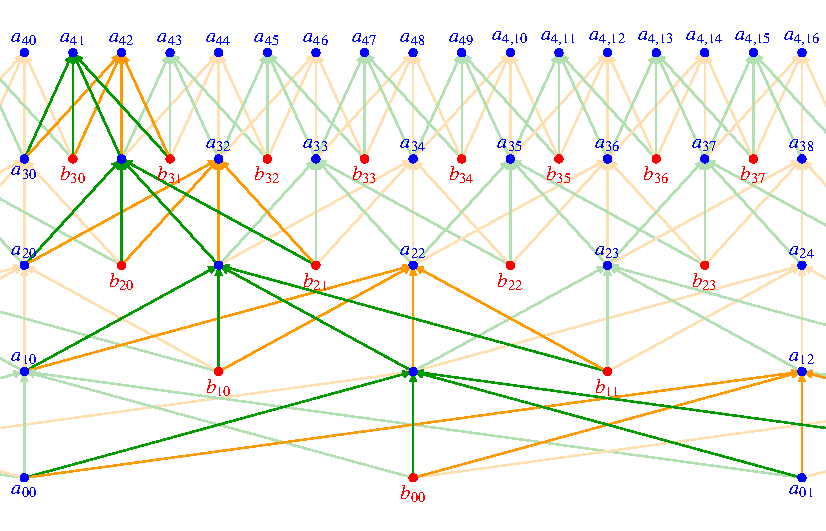
\includegraphics[width=\hsize]{chapters/7-algo/images/rueckalgo.pdf}
\caption{Datenfluss im Rücktransformationsalgorithmus zur in
Abbildung~\ref{algo:image:fastalgo} dargestellten Wavelettransformation.
Die grünen und orangen Pfeile entsprechen farblich den Koeffizienten
in der Rücktransformationsmatrix~\eqref{fast:rueckmatrix} (man beachte
aber, dass in Abbildung~\ref{algo:image:fastalgo} die Koeffizienten mit
Indizes $-1,\dots,2$ von $0$ verschieden waren, daher decken sich die
Pfeile nicht mit der Matrix~\eqref{fast:rueckmatrix}).
Es wird deutlich, dass für die Rücktransformation nur die Detailkoeffizienten
$b_{j,k}$ für alle $j$ und $k$
sowie die ``gröbsten'' Approximationskoeffizienten $a_{0,k}$ benötigt werden.
Das gleiche hierarchische Muster wie in der Wavelettransformation erlaubt
die Synthese ebenfalls in einer Zeit, die linear von der Inputlänge
abhängt.
\label{fast:rueckfluss}}
\end{figure}

\subsection{Schnelle Waveletsynthese}
Die schnelle Wavelettransformation kann mit Hilfe der
Matrix~\eqref{fast:transmatrix}
geschrieben werden.
Die Umkehrtransformation muss daher die transponierte und konjugierte Matrix
\eqref{algo:rueckmatrix} verwenden.
Aus ihr kann man ablesen, wie die Koeffizienten $a_{j+1,k}$ aus $a_{j,k}$
und $b_{j,k}$ berechnet werden können.

\begin{satz}
Die Umkehrtransformation der schnellen Wavelettransformation berechnet die
hochfrequenten Waveletkoeffizienten $a_{j+1,k}$ aus den Koeffizienten
$a_{j,k}$ und $b_{j,k}$ gemäss
\begin{equation}
\begin{aligned}
a_{j+1,k}
&=
\dots
+
h_{k+4}
a_{j,-2}
+
g_{k+4}
b_{j,-2}
+
h_{k+2}
a_{j,-1}
+
g_{k+2}
b_{j,-1}
+
h_{k}
a_{j,0}
+
g_{k}
b_{j,0}
+
h_{k-2}
a_{j,1}
+
g_{k-2}
b_{j,1}
+
\dots
\\
&=
\sum_{l\in\mathbb Z}
h_{k-2l}
a_{j,l}
+
\sum_{l\in\mathbb Z}
g_{k-2l}
b_{j,l}.
\end{aligned}
\end{equation}
\end{satz}

Das Datenflussdiagramm in Abbildung~\ref{fast:rueckfluss} zeigt, 
wie die Detailkoeffizienten $b_{j,k}$ den Approximationen $a_{j,k}$
mehr Information hinzufügen, wodurch die Approximationskoeffizienten
$a_{j+1,k}$ entstehen.
Es liegt die gleiche hierarchische Struktur vor, die den Rechenaufwand
Analysealgorithmus unter Kontrolle hielt. 
Auch die Synthese ist daher in Zeit $O(l)$ von der Inputlänge $l$
möglich.

\begin{beispiel}
Die Koeffizienten $h_{\cdot}$ und $g_{\cdot}$ für das Haar-Wavelet sind
wohlbekannt.
Sie sind $h_0=h_1=1$, $g_0=0$ and $g_1=-1$.
Die zugehörige Transformationsmatrix ist in Abbildung~\ref{algo:haarmatrix}
tabellarisch dargestellt.
\begin{figure}
\begin{equation}
\bgroup
\def\arraystretch{1.5}
\begin{tabular}{>{$}c<{$}|
>{$}c<{$}
>{$}c<{$}
>{$}c<{$}
>{$}c<{$}
>{$}c<{$}
>{$}c<{$}
>{$}c<{$}
>{$}c<{$}
>{$}c<{$}
>{$}c<{$}
>{$}c<{$}
>{$}c<{$}}
          &\dots &a_{j,-2}&b_{j,-2}&a_{j,-1}&b_{j,-1}&a_{j,0}&b_{j,0}&a_{j,1}&b_{j,1}&a_{j,2}&b_{j,2}&\dots \\
\hline
\vdots    &\ddots&\vdots  &\vdots  &\vdots  &\vdots  &\vdots &\vdots &\vdots &\vdots &\vdots &\vdots &\ddots\\
a_{j+1,-2}&\dots &    0   &    0   &    1   &    1   &    0  &    0  &    0  &    0  &    0  &    0  &\dots \\
a_{j+1,-1}&\dots &    0   &    0   &    1   &   -1   &    0  &    0  &    0  &    0  &    0  &    0  &\dots \\
a_{j+1, 0}&\dots &    0   &    0   &    0   &    0   &    1  &    1  &    0  &    0  &    0  &    0  &\dots \\
a_{j+1, 1}&\dots &    0   &    0   &    0   &    0   &    1  &   -1  &    0  &    0  &    0  &    0  &\dots \\
a_{j+1, 2}&\dots &    0   &    0   &    0   &    0   &    0  &    0  &    1  &    1  &    0  &    0  &\dots \\
a_{j+1, 3}&\dots &    0   &    0   &    0   &    0   &    0  &    0  &    1  &   -1  &    0  &    0  &\dots \\
a_{j+1, 4}&\dots &    0   &    0   &    0   &    0   &    0  &    0  &    0  &    0  &    1  &    1  &\dots \\
a_{j+1, 5}&\dots &    0   &    0   &    0   &    0   &    0  &    0  &    0  &    0  &    1  &   -1  &\dots \\
\vdots    &\ddots&\vdots  &\vdots  &\vdots  &\vdots  &\vdots &\vdots &\vdots &\vdots &\vdots &\vdots &\ddots\\
\end{tabular}
\egroup
\end{equation}
\caption{Transformationsmatrix für die Waveletanalyse mit Haar-Wavelet.
In jeder Zeile sind nur zwei Koeffizienten von $0$ verschieden.
\label{algo:haarmatrix}}
\end{figure}
Damit werden die Umkehrformeln für das Haar-Wavelet zu
\begin{align*}
a_{j+1,2k\phantom{+1}}
&= 
a_{j,k} + b_{j,k}
\\
a_{j+1,2k         +1 }
&= 
a_{j,k} - b_{j,k}.
\end{align*}
Die Umkehrformeln sind bis auf die Bezeichnung der Variablen identisch
mit den Formeln für die schnelle Vorwärtstransformation.
\end{beispiel}


%
% rekonstruktion.tex -- Gram-Operator, duale Basis, Rekonstruktionsformel
%
% (c) 2019 Prof Dr Andreas Müller, Hochschule Rapperswil
%
\section{Rekonstruktion
\label{section:rekonstruktion}}
\rhead{Rekonstruktion}






\section*{Übungsaufgaben}
\rhead{Übungsaufgaben}
\uebungsaufgabe{07001}






